
\chapter{Classificação de vulnerabilidades}
\label{chap:classificacao}

	A classificação de vulnerabilidades representa enorme desafio.
	Nos dias de hoje, não existe nenhum padrão aceito globalmente para essa tarefa.
	Ainda assim, já houve vários avanços na área. 
	Existem padrões para enumerar e catalogar vulnerabilidades, bem como propostas
	que podem criar bases para uma classificação que venha a ser aceita pela comunidade.
	Métricas, relativas	à gravidade e ao impacto, também estão disponíveis
	e são empregadas no auxílio às instituições nas tomadas	de decisões.

	
	No trabalho de Seacord e Householder, \cite{Seacord2005}, temos os fatores que motivam a
	busca pela organização das vulnerabilidades em classes:
	\begin{itemize}
		\item{O entendimento das ameaças que elas representam;}
		\item{Correlacionamento de incidentes, de \textsl{exploits} e de artefatos;}
		\item{Avaliação da efetividade das ações de defesa;}
		\item{Descoberta de tendências de vulnerabilidades;}
	\end{itemize}

	
	Vemos, portanto, que a taxonomia\footnote{Ciência da classificação.} das vulnerabilidades
	pode trazer uma série de benefícios para seu entendimento, tratamento e prevenção.
	Nesse capítulo, nosso intuito é abordar a dificuldade nesse processo e apresentar
	os avanços já obtidos nesse sentido.  


	\section{A dificuldade em classificar; estágio já alcançado: enumeração}
		Antes de entrarmos no mérito das vulnerabilidades, é preciso definir
		com precisão dois termos que utilizaremos por todo o capítulo: classificar e enumerar.
		Como veremos, a taxonomia é mais custosa que a enumeração.

		\subsection{Classificar}
			\label{subsec:classificar}
			Como podemos encontrar em \cite{Holanda1975}, classificar implica "distribuir em classes e/ou grupos
			segundo um sistema". Logo, para a classificação, é preciso haver uma metodologia que possa
			separar os itens em estudo em diferentes grupos. A ciência que estuda esse processo
			é chamada taxonomia. Ela é guiada, conforme \cite{Gregio2005_1}, pelos princípios taxonômicos.
			São eles:
			\begin{description}
				\item[Exclusão mútua]
					Um item não podem ser categorizado simultaneamente em dois grupos.
				\item[Exaustividade]
					Os grupos, unidos, incluem todas as possibilidades.
				\item[Repetibilidade]
					Diferentes pessoas extraindo a mesma característica do objeto devem concordar com
					o valor observado.
				\item[Aceitabilidade]
					Os critérios devem ser lógicos e intuitivos para serem aceitos pela comunidade.
				\item[Utilidade]
					A classificação pode ser utilizada na obtenção de conhecimento na área de pesquisa.
			\end{description}

			
			Vemos que os critérios para a taxonomia são exigentes e pressupõem uma metodologia
			cuidadosamente gerada para atendê-los. 

		\subsection{Enumerar}
			A enumeração é um processo semelhante a 
			"indicar por números; relacionar metodicamente"; como encontramos
			em \cite{Holanda1975}.
			Trata-se, portanto, de algo muito mais simples que a classificação.
			Mesmo sendo mais simples, é extremamente importante pois permite
			que os itens enumerados sejam facilmente apontados e diferenciados entre si.
			
			
			Sem um procedimento de enumeração dos objetos de estudo, adotado de comum acordo,
			não é possível que duas partes se comuniquem sem risco de cometerem enganos. 
			Quem garante que estão tratando exatamente da mesma coisa naquele momento?
			Logo a enumeração é essencial para o devido entendimento sobre os objetos
			de estudo.

		\subsection{Da enumeração à classificação}
			No trabalho de Mann, \cite{Mann1999}, há um excelente paralelo entre a
			questão abordada nesse capítulo e o advento da tabela 
			periódica\footnote{Dispõe sistematicamente os elementos de acordo com suas propriedades permitindo
			uma análise multidimensional.} na Química. 
			A organização dos elementos da forma como conhecemos hoje na tabela periódica
			foi um processo longo que culminou com as ideias de Dimitri Mendeleev.
			Outros químicos que o precederam foram responsáveis pela identificação e
			listagem dos elementos. Isso possibilitou um melhor estudo e uma maior
			troca de informação precisa entre os pesquisadores.


			Segundo Mann, a tabela periódica só pode ser efetivamente criada graças
			aos esforços daqueles que enumeraram os elementos de forma mais simples
			antes de Mendeleev. O trabalho deles permitiu a interoperabilidade
			necessária para o surgimento da tabela periódica.
			Da mesma forma, nos anos antecedentes a 2000, a comunidade que estudava
			e acompanhava as vulnerabilidades estava num patamar semelhante àqueles
			que precederam Mendeleev. Ou seja, sequer havia uma enumeração mais
			amplamente aceita e reconhecida das vulnerabilidades que permitisse
			avanços suficientes para uma taxonomia.

			
			Citamos o ano de 2000 como parâmetro, pois nessa época, 1999, surgiria um projeto
			que se tornaria referência para a criação de uma padronização da enumeração
			de vulnerabilidades. Não seria ainda um evento comparável à criação da
			tabela periódica para Química (pois não trouxe a taxonomia) 
			mas certamente lançaria as bases para
			a interoperabilidade exigida para estudos mais aprofundados na área.
			Estamos falando da criação do 
			CVE(Common Vulnerabilities and Exposures)\footnote{http://cve.mitre.org}\footnote{Na época
			de sua criação era originalmente conhecido por Common Vulnerabilities Enumeration - vide
			\cite{Meunier2006} pg. 9.}
			pelo MITRE. A seção \ref{sec:cve} traz mais detalhes.


			Podemos dizer, portanto, que atualmente, embora não tenhamos uma taxonomia
			amplamente aceita pela comunidade, já foi atingido o estágio de enumeração.
			Projetos como o CVE podem ser considerados como marcos dessa etapa.
			A seguir, iremos abordar em mais detalhes o surgimento e o funcionamento dele.
			Isso nos possibilitará compreender melhor a complexidade da classificação
			das vulnerabilidades bem como irá facilitar o entendimento dos capítulos
			seguintes que abordam \textsl{exploits}.
			

	\section{CVE}
	\label{sec:cve}

		\subsection{Surgimento e objetivos}
			Para deixar mais nítida a dificuldade de interoperabilidade
			das organizações no que se refere a ameaças de segurança na época
			que antecede o CVE, temos a tabela \ref{tab:torre_babel}, extraída de \cite{Martin2001}.
			Ela	mostra como diferentes organizações se referiam à mesma vulnerabilidade
			em 1998. Trata-se de um verdadeira Torre de Babel.

			\begin{table}
				\begin{tabular}{|l|c|c|}
					\hline
						\textbf{Organização} & \textbf{Como se referia à vulnerabilidade}\\
					\hline
						CERT & CA-96.06.cgi\_example\_code\\
					\hline
						Cisco Systems & http - cgi-phf\\
					\hline
						DARPA & 0x00000025 = http PHF attack\\	
					\hline
						IBM ERS & ERS-SVA-E01-1996:002.1\\	
					\hline
						Security Focus & \#629 - phf Remote Command Execution Vulnerability\\	
					\hline
				\end{tabular}
				\caption{Uma vulnerabilidade: diversos nomes e nenhum entendimento}\label{tab:torre_babel}
			\end{table}
			

			O CVE, como dito anteriormente, surge em 1999 e seu maior objetivo, como podemos
			ler em sua FAQ, \cite{CVE2010}, é tornar mais fácil
			o compartilhamento de informações sobre vulnerabilidades utilizando uma enumeração comum.
			Essa enumeração é realizada através da manutenção de uma lista na qual, conforme
			encontramos em \cite{Santos2004}, valem os seguintes princípios:
			\begin{itemize}
				\item{Atribuição de um nome padronizado e único a cada vulnerabilidade.}
				\item{Independência das diferentes perspectivas em que a vulnerabilidade ocorre.}
				\item{Abertura total voltada ao compartilhamento pleno das informações.}
			\end{itemize}


			Segundo a própria organização, vide \cite{CVE2010}, o CVE não possui um objetivo 
			inicial de conter alguma espécie de taxonomia. Essa é considerada uma área de pesquisa
			ainda em desenvolvimento. É esperado que, com o auxílio prestado pela
			catalogação das vulnerabilidades já constitua um importante passo para que
			isso ocorra.

			\begin{figure}
				\begin{center}
					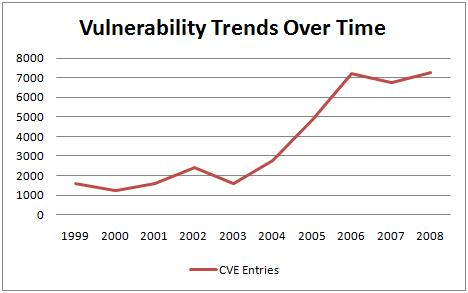
\includegraphics[width=0.65\textwidth]{vulnerabilidades_CVE.jpg}
					\caption{Vulnerabilidades registradas no CVE a cada ano entre 1999 e 2008.
							Fonte: \cite{Florian2009}}
					\label{fig:vulnerabilidades_CVE}
				\end{center}
			\end{figure}

			
			Na figura \ref{fig:vulnerabilidades_CVE}, podemos visualizar um histórico
			da quantidade de vulnerabilidades adicionadas. Nos últimos anos podemos
			perceber que os incidentes registrados ficam na média de 7000.
			Isso mostra relevância que o projeto do CVE alcançou.
			
			 
		
		\subsection{Funcionamento}
			O CVE é formado por uma junta de especialistas em segurança dos meios acadêmico, comercial e
			governamental. Eles são responsáveis por analisar e definir o que será feito dos reports passados
			pela comunidade - se eles devem ou não se integrar àqueles já pertencentes à lista.
			Cabe a eles definir nome, descrição e referências para cada nova ameaça.


			Esse processo inicia quando uma vulnerabilidade é reportada.
			Ela assume um CAN (Candidate Number), número de candidata.
			Até que ela seja adicionada à lista, ele permanece com um CAN que
			a identificará. Apenas após o devido estudo e aprovação do caso pela junta
			responsável, é que ela assume um identificador CVE.

			
			Os identificadores CVE são definidos conforme o padrão: CVE-2010-0021.
			Onde, separados por '-', há 3 partes. A primeira é fixa: CVE.
			A segunda refere-se ao ano de surgimento; enquanto a terceira
			indica o número sequencial daquela vulnerabilidade entre todas
			aquelas que foram adicionadas naquele ano. Logo, no exemplo fornecido,
			essa seria a vigésima primeira de 2010.
		
			
			Uma vez integrada, a vulnerabilidade passa a estar publicamente disponível.
			Essa abertura pode servir de auxílio aos atacantes - pois informações
			sobre possíveis furos de segurança são sempre bem vindas a eles.
			Porém, conforme podemos verificar na FAQ do CVE, \cite{CVE2010}, há uma série
			de motivos pelos quais a disponibilidade desses dados supera o risco
			oferecido pela exposição. São eles:
			\begin{itemize}
				\item{O CVE está restrito a publicar vulnerabilidades já conhecidas.}
				\item{Por diversas razões, a comunidade de segurança de informação
					sofre mais para compartilhar dados sobre as ameças
					que os atacantes.}
				\item{É muito mais custo a uma organização proteger toda sua rede
					contra as ameças que a um atacante descobrir e explorar uma delas para
					comprometer alguma das redes.}
			\end{itemize}
			
		
	\section{Propostas taxonômicas}
		\label{sec:prop_taxonomicas}
		Nessa Seção, apresentaremos taxonomias para vulnerabilidades e um projeto, análogo ao CVE,
		que reúne esforços para a padronização da classificação: o CWE.
		Primeiramente, faremos um breve histórico das propostas já criadas com esse fim.
		A seguir, apresentaremos algumas das classificações que consideramos de maior relevância
		e, por fim, trataremos do projeto CWE - que assume importante papel no contexto atual
		na catalogação dos tipos de vulnerabilidades existentes.

		\subsection{Histórico das propostas}
		\label{subsec:historico_prop_taxonomicas}
			Em \cite{Gregio2005}, encontramos um levantamento das 
			dessas alternativas. Mas, como veremos, nenhuma delas atinge os objetivos
			de uma taxonomia plena - apresentados na seção \ref{subsec:classificar}.
			Assim, buscaremos discutir as ideias para as metodologias
			de classificação com o intuito de apontar suas vantagens e fraquezas.

			Em 1976, surge o primeiro estudo, chamado \textsl{Research Into Secure Operating Systems}(RISOS).
			Ele objetivava auxiliar na compreensão das falhas encontradas nos sistemas operacionais
			como MUTICS, GECOS, IBM OS. Foram propostas 7 classes, pág. 328 de \cite{Gregio2005}:
			\begin{itemize}
				\item{Validação incompleta de parâmetros;}
				\item{Validação inconsistente de parâmetros;}
				\item{Compartilhamento implícito de privilégios ou dados confidenciais;}
				\item{Validação assíncrona ou serialização inadequada;}
				\item{Autorização, autenticação ou identificação inadequadas;}
				\item{Violação de proibição de limite;}
				\item{Erro de lógica explorável;}
			\end{itemize}
			Esse estudo teve importância pelo pioneirismo, mas se limitava a problemas
			de sistemas operacionais bem como não atendia a todos os princípios taxonômicos.

	
			Dois anos após o projeto RISOS, em 1978, seria criado o \textsl{Protection Analysis}(PA).
			Seu objetivo principal era permitir que qualquer pessoa, mesmo sem conhecimento
			específico sobre falhas de segurança, utilizando um padrão dirigido, pudesse
			encontrar vulnerabilidades nos sistemas - \cite{Katrina2005}, pág. 2.
			O PA, separava as falhas em 4 grandes classes - \cite{Gregio2005}, pág. 329:
			\begin{itemize}
				\item{Reforço e inicialização do domínio da proteção;}
				\item{Validação de operandos / dependências no gerenciamento das filas;}
				\item{Sincronização imprópria;}
				\item{Erros de seleção de operadores críticos;}
			\end{itemize}
			Embora a ideia inicial do PA também incluísse a detecção automática de vulnerabilidades,
			sendo pioneiro nesse ponto, a classificação proposta não era intuitiva e de difícil aplicação -
			conforme consta em \cite{Katrina2005}. Logo, a aplicação prática não foi levada adiante, mas
			a base da proposta adicionou conhecimento na área.


			Segundo \cite{Gregio2005}, apenas no ano de 1992, teríamos uma nova proposta
			de classificação que trouxesse nova perspectiva ao estudo em questão.
			Trata-se do trabalho de Landwher: \textsl{A Taxonomy of Computer Security Flaws}.
			Seu foco estava no auxílio aos projetistas no desenvolvimento mais seguro do software.
			Sua classificação tinha por base 3 critérios:
			\begin{itemize}
				\item{Como o defeito entra no sistema(gênese);}
				\item{Quando o defeito entrou no sistema(tempo de introdução);}
				\item{Onde ele se manifesta(localização);}
			\end{itemize}
			De acordo com Grégio, seu principal problema era a ambiguidade no processo de classificação.
			A dependência na visão do classificador tem do sistema impede a objetividade necessária
			a uma boa taxonomia.
			Outro problema nessa proposição, abordado por Katrina, em \cite{Katrina2005}, está
			na dificuldade que pode surgir caso, por exemplo, se desconheça a forma como a vulnerabilidade
			adentrou o sistema. Em tal situação, não seria possível identificar a gênese.
			
			
			No ano de 1996, a taxonomia proposta por Aslam, em \textsl{Use of a Taxonomy of Security Faults},
			traria nova acréscimo às pesquisas na área. Segundo, \cite{Katrina2005}(pág. 3), o esquema
			proposto por Aslam é bastante preciso; consistindo numa série de perguntas para cada
			categoria de vulnerabilidade. Em \cite{Gregio2005}, pág. 329, encontramos as 
			classes criadas por Aslam, com suas subdivisões:
			\begin{enumerate}
				\item{Falhas de codificação;}
					\subitem{Erros de sincronização;}
					\subitem{Erros na validação de condição;}
				\item{Falhas emergentes;}
					\subitem{Erros de configuração;}
					\subitem{Falhas no ambiente;}
			\end{enumerate}
			Embora seja uma taxonomia precisa, conforme ressaltado anteriormente, ela sofre
			por estar focada excessivamente em sistemais UNIX - como indicado em \cite{Katrina2005}.
			

		\subsection{Taxonomias e classificações mais recentes}
		\label{subsec:prop_taxonomicas_recentes}
			Agora trataremos das propostas para classificação de vulnerabilidades que surgiram
			mais recentemente (após 2005) e que merecem uma análise mais apurada. São eles:
			\begin{itemize}
				\item{\textsl{Preliminary List of Vulnerability Examples for Researchers}(PLOVER);}
				\item{\textsl{Comprehesive, Lightweight Application Security Process}(CLASP);}
				\item{\textsl{Seven Pernicious Kingdoms};}
			\end{itemize}
			São taxonomias que não passam pelo rigor científico, pois não atendem a todos
			os princípios taxonômicos, mas que ainda assim acrescentam bastante sobre o
			entendimento dos problemas que as vulnerabilidades representam. É o que
			diz Meunier em \cite{Meunier2006} ao tratar das classificações populares.


			O PLOVER, criado em 2005 pelo MITRE em colaboração com o 
			DHS(\textsl{US. Departement	of Homeland Security})\footnote{http://www.dhs.gov/index.shtm} e o
			o NIST(\textsl{National Institute of Technology}) é um esquema de classificação
			que possui dezenas de categorias principais e, naturalmente, possui ainda mais precisão
			do que a proposição de Aslam. Um de seus principais idealizadores foi Steve Christey.
			Trata-se de um trabalho com sólidas fundações, pois
			apresenta um \textsl{Framework} conceitual que permite discutir as vulnerabilidades
			em diversos níveis. Nele são definidos uma série de conceitos essenciais
			para o estudo da área. Pode ser encontrado em detalhes em \cite{Christey2006}.
			

			Dentre as suas contribuições, destacam-se o caráter prático; mais de 1400 vulnerabilidades
			identificadas no CVE foram devidamente classificadas utilizando esse sistema.
			Foi uma taxonomia construída de baixa para cima(\textsl{bottom-up}).
			Essa experiência foi muito útil para a definição dos critérios.


			Abaixo, seguem algumas categorias de mais alto nível existentes no PLOVER
			(existem 30 no total):
			\begin{description}
				\item[BUFF]{Contém erros como \textsl{Buffer Overflow} e \textsl{Heap Overflow}.}
				\item[SPECTS(\textsl{Technology-Specific Special Elements})]{Abrange erros que possibilitam
					ataques de Injeção de SQL e XSS.}
				\item[RACE]{Erros advindos de condições de corrida.}
				\item[CRYPTO]{Falhas relacionadas o uso inadequado ou problemas na criptografia.}
			\end{description}
			Conforme será abordado a seguir, o PLOVER serviu de base para a criação do projeto CWE.

			

			Do trabalho de John Viega e outros colaboradores, temos o CLASP. É um conjunto
			de atividades que busca melhorar a segurança dos sistemas. Embora
			trate também da classificação das falhas, ele vai muito além. Possui uma formalização
			de boas práticas para a construção de software seguro através de ciclos de desenvolvimento
			estruturados, repetíveis e mensuráveis - \cite{Secure2006}.
			

			No que se refere à classificação, sua contribuição tem origem no trabalho proposto por 
			Landwher(que utiliza os critérios de gênese, tempo de introdução e localização).
			O CLASP adiciona outro eixo classificatório: a consequência.
			As classes mais básicas, tipo do problema, são:
			\begin{itemize}
				\item{Erros de \textsl{range} e de tipo;}
				\item{Problemas no ambiente;}
				\item{Erros de sincronização e de temporização;}
				\item{Erros de protocolo;}
				\item{Erros de lógica;}
				\item{\textsl{Malware};}
			\end{itemize}
			Para exemplificar, consideremos uma falha que permita um \textsl{Buffer overflow}.
			Segundo o CLASP, trata-se de um erro de tipo e de \textsl{range} - já
			que é permitida a escrita além do permitido no \textsl{buffer}. A injeção de SQL
			também cai na mesma categoria, pois os dados passados pelo usuário são utilizados
			incorretamente; permitindo que assumam um tipo inesperado. Já um erro no qual é ignorado
			o valor de retorno de uma função é considerado como erro de lógica - como, por exemplo,
			uma chamada à função malloc que não avalia se a alocação de memória foi bem sucedida.


			
			O \textsl{Seven Pernicious Kingdoms}, de autoria de Katrina Tsipenyuk et alem, conforme
			\cite{McGraw2006}, capítulo 12, é uma taxonomia que, mesmo sendo imperfeita possibilita
			um bom entendimento por parte dos desenvolvedores; auxiliando na prevenção de problemas.
			É estruturada em dois conjuntos emprestados da Biologia: Filo e Reino.
			O Reino é a classificação mais ampla - enquanto o Filo é uma subdivisão do Reino.
			Possui 8 reinos; procurando respeitar a famosa regra de George Miller 
			do "sete mais ou menos dois"\footnote{Artigo 
			\textsl{The Magic Number Seven, Plus or Minus Two} de George Miller.}. São eles:
			\begin{description}
				\item[Erro de validação e de representação]{Resultam da confiança
					indevida nos dados de entrada. Caso do \textsl{Buffer Overflow},
					injeção de SQL, XSS.}
				\item[Abuso de API]{Sendo a API um contrato entre quem chama a rotina
					e aquela que é chamada, uma quebra das regras pode resultar em problemas de segurança.
					Quando quem chama uma função assume certas condições que não estão garantidas
					pela rotina chamada, temos um caso de abuso de API.}
				\item[\textsl{Features} de segurança]{Trata do uso correto de peças chave na
					garantia da segurança do software como: criptografia, autenticação, gerenciamento
					de privilégios, entre outros.}
				\item[Tempo e estado]{Relativo a problemas advindos do paralelismo. Como erros
					na sincronização que expõem o sistema.}
				\item[Gerenciamento de erros]{Vulnerabilidades desse reino surgem quando
					os erros não tratados corretamente. Quando um erro expõe informações
					do sistema ao atacante desnecessariamente, já estamos diante de um exemplo.}
				\item[Qualidade de código]{Se a qualidade é baixa, o comportamento é imprevisível.
					Tendo em vista essa regra, problemas na codificação acabam levando
					a erros que permitem a subversão do sistema.}
				\item[Encapsulamento]{Falhas relacionadas ao não estabelecimento de limites entre os 
					componentes do sistema.}
				\item[Ambiente]{Trata de problemas surgidos com questões externas ao software.
					Não estão relacionados ao código, mas influenciam diretamente na segurança.}
			\end{description}
			
			
			Como subdivisões dos reinos, encontramos, por exemplo, o filo correspondente ao
			\textsl{Buffer Overflow} - no reino do Erro de Validação e de Representação.
			Ainda nele, também encontramos o filo de Injeção de Comandos.			
			Já no reino de \textsl{Features de segurança}, está o filo da Randomização Insegura -
			que trata da randomização incorreta que pode ser uma fraqueza para a criptografia.
			O erro correspondente a NULL \textsl{pointer} pertence ao filo \textsl{Null Dereference} -
			que por sua vez é englobado pelo reino Qualidade de código.
			

			Essa classificação foi desenvolvida com a projeção da adição de novos filos
			conforme a necessidade. O intuito foi de criar reinos amplos o suficiente para que
			os devidos filos fossem incorporados com o tempo.

		
		\subsection{O projeto CWE}
			\label{subsec:cwe}
			Após o surgimento do CVE, uma padronização para identificação das vulnerabilidades
			foi sendo alcançada. Entretanto, a classificação, que não era objetivo direto do CVE,
			foi deixada de lado pelo projeto. Em 2005, mais de 5 anos depois da criação do CVE, 
			após o estudo de uma série de vulnerabilidades catalogadas, foi 
			gerado o PLOVER - abordado na Seção anterior.
			

			A partir do estudo e da classificação resultante do PLOVER, surgiu a possibilidade
			de se estabelecer descrições comuns a comunidade para os tipos de vulnerabilidades.
			Desse esforço, surge o CWE: \textsl{Common Weakness Enumeration}\footnote{http://cwe.mitre.org/}.
			Embora esteja fundamentada na classificação proposta pelo PLOVER, o CWE não se limita
			a ela. Também opera com outras como: \textsl{Seven Pernicious Kingdoms} e o CLASP.

			
			Conforme encontramos em \cite{CWEAbout}, ele é uma resposta à necessidade das instituições
			e das organizações em utilizarem os mesmos termos e taxonomias no tratamento dos
			problemas de segurança que enfrentam. Como saber quais as classes de vulnerabilidades
			que uma ferramenta de detecção é capaz de encontrar? Perguntas como essas caem justamente
			no escopo do CWE.
			

			Entre os objetivos e impactos diretos do CWE, encontrados em \cite{CWE2009}, temos:
			\begin{itemize}
				\item{Providencia uma linguagem comum para as discussões relativas às fraquezas
					encontradas no software e nos sistemas;}
				\item{Permite aos fabricantes de ferramentas de segurança fazer afirmações
					claras e consistentes sobre quais tipos de falhas elas cobrem;}
				\item{Permite aos compradores de ferramentas de segurança comparar
					com melhor qualidade as alternativas em virtude da discriminação
					da cobertura delas encontradas no CWE.}
				\item{Habilita governos, instituições e a indústria a utilizar a padronização
					fornecida pelo CWE para estabelecer contratos, termos e condições.}
			\end{itemize}

			
			Mesmo tendo sido criado recentemente, tendo menos de 5 anos completos, o projeto do 
			CWE certamente já está trazendo	contribuições para a padronização na área de 
			classificação de vulnerabilidades.
			A esperança é que ele se fortalece e possibilite uma referência de grande valor
			assim como foi estabelecido com o CVE.


	\section{Métricas para vulnerabilidades: CVSS}
		Comparar objetivamente vulnerabilidades de acordo com sua criticidade é
		algo muito útil para as organizações.
		Isso possibilita que os gestores mensurem o grau de urgência com que devem
		ser tratadas as ameaças. Podemos considerar esse procedimento
		como um tipo rudimentar de classificação. Ainda que não seja uma taxonomia,
		assume um papel de destaque por permitir um padrão para distinguir
		vulnerabilidades mais graves das demais.

		\subsection{Surgimento do CVSS}
			Para essa finalidade existe uma alternativa relativamente recente, o CVSS
			(Common Vulnerability Scoring System), criado em 2005. 
			Trata-se de um \textsl{framework} aberto para atribuição de escore a vulnerabilidades.
			Ele oferece as seguintes vantagens, encontradas em \cite{Mell2007} - pg. 3:
			\begin{description}
				\item[Padronização de escore de vulnerabilidades]{Quando uma organização normaliza
				os escores de vulnerabilidades em todas suas plataformas de hardware e software,
				ela pode instituir uma política comum de gerenciamento das ameaças.}
				\item[\textsl{Framework} aberto]{A abertura permite que os usuários tenham
				livre acesso para compreenderem as razões das vulnerabilidades assumirem
				esse ou aquele escore.}
				\item[Priorização de riscos]{Quando o escore ambiental é calculado, a vulnerabilidade
				passa a possuir contexto. De tal forma que o risco real que ela representa
				para a organização possa ser mensurado.}
			\end{description}

			
			A organização responsável pelo CVSS é a 
			\textsl{Forum of Incident Response and Security Teams} (FIRST)\footnote{www.first.org}.
			Além do FIRST, as seguintes organizações também cooperaram para seu surgimento:
			\begin{itemize}	
				\item{CERT/CC}
				\item{Cisco}
				\item{DHS/MITRE}
				\item{eBay}
				\item{IBM Internet Security Systems}
				\item{Microsoft}
				\item{Qualys}
				\item{Symantec}
			\end{itemize}	
			Sua primeira versão data de 2005. Desde 2007, já se encontra na segunda versão;
			tratada em \cite{Mell2007}. Nesse trabalho, abordaremos	apenas a versão atual do CVSS.

		\subsection{As métricas usadas}
		\label{subsec:metricas_cvss}
			Para o cálculo do escore de uma vulnerabilidade, o CVSS, na sua versão 2, possui diversas métricas
			que são divididas em 3 grupos principais. 
			em \cite{Mell2007}\footnote{Termos em inglês traduzidos livremente pelo autor.}:
			\begin{description}
				\item[Métricas básicas]{Representam as características fundamentais da vulnerabilidade
				e são constantes com relação ao tempo e ao ambiente.}
				\item[Métricas temporais]{Mudam com o transcorrer do tempo, mas não são suscetíveis
				a fatores ambientais.}
				\item[Métricas ambientais]{Estão relacionadas unicamente ao ambiente em que a vulnerabilidade
				é analisada. Por isso, são absolutamente dependentes das particularidades de cada caso.}
			\end{description}	
			Na tabela \ref{tab:grupos_cvss}, são mostradas as métricas usadas subdivididas nos seus respectivos
			grupos. 

			\begin{table}
				\begin{tabular}{|c|c|c|}
					\hline
					\multicolumn{3}{|c|}{ \textbf{CVSS} } \\
					\hline
					\textbf{Métricas básicas} & \textbf{Métricas Temporais} & \textbf{Métricas Ambientais} \\
					\hline
					Vetor de acesso & Facilidade de exploração & Dano colateral potencial \\
					Complexidade de acesso & Confiabilidade no \textsl{report} & Abundância de alvos\\
					Necessidade de autenticação & Nível de remediação & Importância da confidencialidade \\
					Impacto na confidencialidade & & Importância da integridade\\
					Impacto na integridade & & Importância da disponibilidade \\
					Impacto na disponibilidade & &  \\
					\hline
				\end{tabular}
				\caption{Métricas CVSS por grupo}\label{tab:grupos_cvss}
			\end{table}
			
			
			A seguir, faremos breve explicação de cada uma das métricas dos três grupos - vide
			tabela \ref{tab:grupos_cvss}.
			Para o grupo \textbf{básico}, existem seis critérios. São eles:
			\begin{description}
				\item[Vetor de acesso]{Diz respeito ao nível de acesso necessário para explorar
					a vulnerabilidade. Pode assumir três valores: 
					\textbf{Local}(exige acesso físico ou uma conta \textsl{shell}), 
					\textbf{Rede adjacente}(é preciso ter acesso à rede local)
					ou \textbf{Rede}(indica a chamada vulnerabilidade \textsl{remota} - pode ser disparada
					de qualquer ponto da Internet).}
				\item[Complexidade de acesso]{Indica a complexidade a ser enfrentada
					pelo atacante para que ele, uma vez que tenha obtido acesso ao sistema alvo,
					possa explorar a vulnerabilidade. Assume um dos valores \textbf{alto, médio ou baixo}.
					A complexidade é considerada alta, por exemplo, se o ataque exige alguma
					técnica de engenharia social mais sofisticada ou se existe uma condição de corrida
					com janela muito exígua que deve ser vencida.}
				\item[Necessidade de autenticação]{Mede a quantidade de vezes que o atacante
					é obrigado a se autenticar durante o ataque - mesmo que seja usada a mesma credencial.
					É um dos valores: \textbf{nenhuma, uma, várias}}.
				\item[Impacto na confidencialidade]{Mede o impacto causado
					na abertura de dados confidenciais gerados pelo ataque.
					Se nenhuma informação, em princípio protegida, é comprometida a medida
					assume valor \textbf{nenhum}. Havendo acesso a alguma informação, é considerado
					\textbf{parcial}. É dito \textbf{completo} caso o atacante tenha total acesso
					de leitura aos dados confidenciais.}
				\item[Impacto na integridade]{Avalia a possibilidade que o atacante
					possui de alterar os dados quando o ataque é bem sucedido.
					Se não é mais possível confiar na integridade dos dados após o ataque,
					pois qualquer arquivo pode ter sido modificado, é considerada \textbf{completa}.
					Não havendo possibilidade de alteração, assume o valor \textbf{nenhuma}.
					É denominada \textbf{parcial} quando apenas parte dos dados
					pode ter sido comprometidos.}
				\item[Impacto na disponibilidade]{Indica o quanto a disponibilidade do sistema
					pode ser afetada pelo ataque. É dita \textbf{completa} caso o sistema
					possa ser totalmente desligado ou inutilizado pelo atacante. Assume o valor
					\textbf{nenhuma} quando não pode haver alteração na disponibilidade e
					\textbf{parcial} se o serviço ainda puder estar disponível mas não plenamente.}
			\end{description}
			

			As métricas do grupo \textbf{temporal} são opcionais. Ou seja, podem ser
			desconsideradas no cálculo do escore conforme a vontade nos analistas.
			Por isso, cada uma delas pode assumir o valor \textbf{não definido} indicando
			que ela não deve participar do escore.
			São 3 os critérios que são suscetíveis a alterações com o passar do tempo:
			\begin{description}
				\item[Facilidade de exploração]{Mede o estado atual das técnicas
					e do código disponível para exploração da vulnerabilidade.
					Seus valores são, em ordem crescente de facilidade: 
					\textbf{não comprovada},  \textbf{prova de conceito},
					\textbf{funcional} e \textbf{alta}.
					O primeiro indica que um \textsl{exploit} é meramente teórico
					e não há código disponível que comprove como explorar a falha.
					Havendo código facilmente acessível de \textsl{exploit}
					ou mesmo se operações manuais são suficientes, estamos
					diante de alta facilidade de exploração.}
				\item[Confiabilidade no \textsl{report}]{
					Mede o grau de confiança na existência da vulnerabilidade
					bem como a credibilidade dos detalhes técnicos fornecidos
					quando ela foi reportada. Seus possíveis valores são:
					\textbf{não confirmada}(quando há apenas um rumor de uma origem
					sem credibilidade), \textbf{não corroborada}(há fontes não oficiais
					com possíveis incoerência em seus \textsl{reports}) e \textbf{confirmada}(
					o autor ou o fabricante admitem o problema ou ele já é amplamente
					conhecido existindo até \textsl{exploits} facilmente encontrados).
					}
				\item[Nível de remediação]{Determina o quão longe se está de uma medida
					definitiva para estancamento da vulnerabilidade.
					Logo que o problema surge, assume o valor \textbf{indisponível}.
					Se houver alguma forma, não oficial, de mitigar a vulnerabilidade,
					é dito que a remediação está no estágio de 	\textbf{\textsl{workaround}}.
					Se existe alguma medida oficial, mas ainda não definitiva, 
					seu valor é \textbf{conserto temporário}. O nível é máximo,
					portanto assumindo o escore mínimo,
					\textbf{conserto definitivo}, caso exista uma remediação de caráter
					oficial definitiva.}
			\end{description}



			Os fatores relativos à influência do ambiente, são medidos na \textbf{métricas
			ambientais}. Cada organização pode sofrer diferentemente o impacto de uma
			vulnerabilidade dada a heterogeneidade com que podem se organizar em termos
			do software e hardware utilizados para desempenhar suas funções.
			Exemplificando, caso uma empresa preste algum tipo de serviço de \textsl{backup} de
			dados, a integridade e a confidencialidade da informação que ela mantém
			possuem importância máxima. Em contrapartida, se a atividade desempenhada pela
			empresa estiver relacionada à hospedagem de projetos de código fonte aberto,
			a disponibilidade assume muito maior importância que a confidencialidade.
			Da mesma forma como os critérios temporais, eles podem assumir o valor não definido;
			indicando que ele não é utilizado no cálculo do escore final.
			Abaixo, são explicados os 5 critérios que compõem a métrica temporal:
			\begin{description}
				\item[Dano colateral potencial]{
					Mede o potencial do estrago que a vulnerabilidade pode causar à organização.
					Podem ser danos patrimoniais, pessoais ou relativos a ganhos financeiros.
					Assume os valores(do menor para o maior dano potencial):
					\textbf{nenhum}, \textbf{baixo}, \textbf{baixo-médio}, \textbf{médio-alto} e
					\textbf{alto}}.
				\item[Abundância de alvos]{Mensura a proporção dos possíveis alvos
					sobre o contingente de sistemas da organização.
					Pode ser \textbf{nenhuma}, \textbf{baixa}(1 a 25\%), 
					\textbf{média}(26 a 75\%) e \textbf{alta}(76 a 100\%)
					.}
				\item[Importância da confidencialidade]{Indica a relevância da
					confidencialidade dos dados mantidos pela empresa. Assume os valores
					\textbf{baixo}, \textbf{médio} e \textbf{alto}.}
				\item[Importância da integridade]{Análogo à importância da confidencialidade.}
				\item[Importância da disponibilidade]{Análogo à importância da confidencialidade.}
			\end{description}
		

		\subsection{Cálculo do escore}
			Tendo sido apresentadas as métricas, faremos breve explicação
			do funcionamento do cálculo do escore,
			que varia de 0 a 10, para uma vulnerabilidade.
			A figura \ref{fig:cvss_metricas_equacoes} apresenta uma visão geral desse processo. 
			\begin{figure}
				\begin{center}
					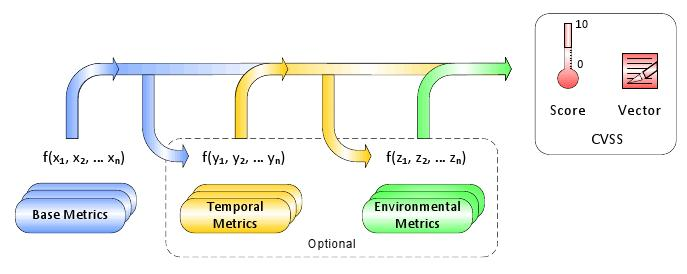
\includegraphics[width=0.85\textwidth]{cvss_metricas_equacoes.jpg}
					\caption{Aplicação das métricas e equações do CVSS. Fonte: \cite{Mell2007}}
					\label{fig:cvss_metricas_equacoes}
				\end{center}
			\end{figure}
			Passos necessários:
			\begin{enumerate}
				\item{Para cada um dos critérios descritos na Seção \ref{subsec:metricas_cvss},
					atribuir um valor válido.}
				\item{Consultar as tabelas, no apêndice	\ref{chap:equacoes_cvss},
					para definir um valor numérico a partir do valor nominal escolhido no passo anterior.}
				\item{Fazer o cálculo do escore básico usando a equação \ref{eq:basica}.
					Para isso, é necessário resolver antes as equações \ref{eq:explorabilidade} e
					\ref{eq:impacto} antes.}
				\item{Fazer o cálculo do escore temporal usando sua respectiva equação - \ref{eq:temporal} -
					 e o escore básico.	Passo opcional. É possível manter apenas o escore básico como o final.}
				\item{Calcular o do escore final usando a equação ambiental, \ref{eq:ambiental},
					 a partir do escore temporal. Também é opcional; pois os critérios 
					ambientais podem ser desconsiderados.}
			\end{enumerate}
			
			
			Ao final do cálculo, a vulnerabilidade recebe um escore de 0 a 10.
			Sendo 10 o valor da mais crítica possível. É importante destacar, que a atribuição
			dos valores, feita no passo 1, deve ser realizada por especialistas na área seguindo
			um critérios padronizados.

			
